\documentclass[a4paper,13pt]{article}
\usepackage[utf8]{inputenc}
\usepackage[english]{babel}
\usepackage{graphicx,subfigure}
\usepackage[top=1in,bottom=1in,left=1in,right=1in]{geometry}
\usepackage{fontspec} %使用非latex字体要使用此包
\setmainfont{WenQuanYi Zen Hei} 

%文档
\begin{document}
\title{HJD Type Crane PLC transformation in control circuit \\HJD型克令吊控制电路的PLC改造}
\author{Yan Peng}
\date{}
\maketitle 
\noindent %不缩进
HJD type crane is commonly used in domestic ships. Its motor is AC three-speed squirrel cage type with three independent sets of the stator windings, the respective number of poles is 4/8/28, and the asynchronous speed is 1500/750/215 r/min. The 4-pole and 8-pole are designed based on constant power. The 4-pole is high-speed pole while 8-pole is rated pole. The 28-pole is low speed pole with low starting current, large starting torque, in order to meet the requirements of frequent starting and landing goods with low speed. Traditional HJD crane control circuit adopts relays and contactors for secondary circuit control. The coils and contacts are easily burned after long-term use, frequently causing accidents. The chief aim of the present work is provide a available way shifting to PLC control reducing the use of coils and contactors. In this paper, The PLC reconstruction, including basic protection control process, rose and fall process, brake process, low/medium/high-speed process, has been supplied. There are no failures in experiment after long-term use. PLC used in this paper is Siemens S7-200.
%插入控制电路图
\begin{figure}[h]  %控制单张图片位置h
\centering
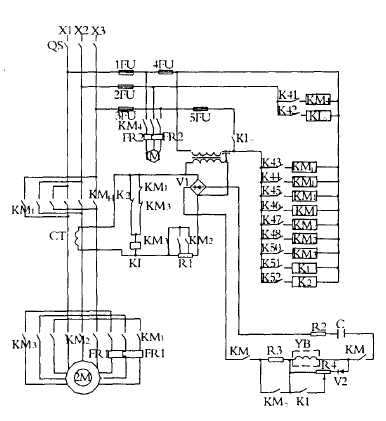
\includegraphics[width=0.6\textwidth]{circuit.png} 
\caption{Control Circuit}
\end{figure}

\begin{enumerate} %列表
\item Reconstruction of Basic Protection Control Process\\
Close the main circuit power and master controller power switch, open the throttle switch and control circuit power switch. In normal circumstances when the protection equipment releases, the energy flow circulates, crane functions correctly. The pictures below realize the reconstruction of fan motor overload protection, the motor windings overheating protection, power supply missing phase protection, emergency forced running and so on. Power Switch I0.1 can also be used as emergency-off switch. Switch I1.4 is zero-voltage switch, The master controller must be put back to zero position when power failure occurred. \\
\item Reconstruction of Rose and Fall Process \\
The process realizes the function of rise and fall, at the same time achieves reverse torque control. Torque control function is based on "automatic parking" and "automatic delay start". Steering control contactors Q0.2, Q0.3 interlock, to avoid short circuit. 
\item Reconstruction of Brake Process \\
The process implements the parking brake as well as automatic grade braking at high speed. In normal rise or fall state, parking brake coil pulls in, while main switch placed on an empty file, brake coil pulls out after delay, mechanical parking brake operates. When the motor parks in medium/high gear, DC master switch disconnect, low speed winding connects, producing rotating magnetic field in the stator, while the rotor still runs at a high speed, so that the motor runs on electrical braking mode.
\item Reconstruction of Low/Medium/High-Speed Process \\
Crane motor runs at low speed after control circuit power closes, so the essence of low-speed process is to close rise or fall contactor, let the crane go in the running state. The medium speed switch locks with low speed switch and interlocking with high speed switch. Compared with medium-speed process, high speed process additionally need to consider the delay from medium-speed to high-speed and heavy load. Heavy load is detected by load relay, when load relay coil pulls in, high speed link cuts, so crane still operates in medium-speed. Taking into account the mandatory run, the medium/high-speed link joins the fan contactor and braking contactor. \\
\item Wiring Diagram and Control Logic Diagrams \\
%插入接线图和控制逻辑图
\begin{figure}[!ht]  %控制多图片位置
\centering
\subfigure[Wiring Diagram]{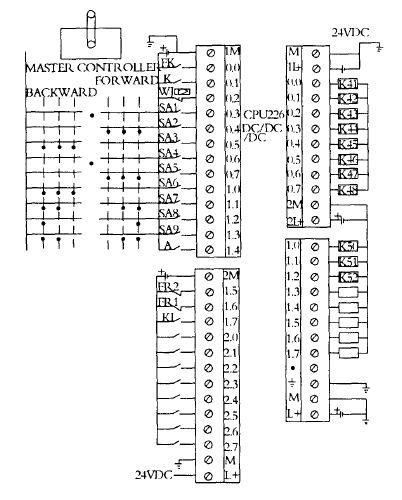
\includegraphics[angle=0,width=0.4\textwidth]{wire.png}}
\subfigure[Logic Diagram]{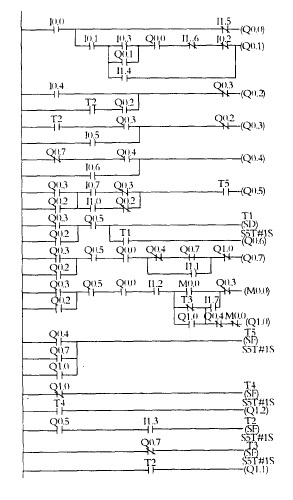
\includegraphics[angle=0,width=0.4\textwidth]{logic.png}}
\caption{The Notification System} %总图名
\end{figure}
\end{enumerate}

%参考文献
\begin{thebibliography}{9}

\bibitem{PL}
T.P. Blackburn, A.J. Cross, C. Hille, P. Slater. "\emph{Neuroscience}", Volume 27, Issue 2, November 1988, Pages 497-506
\bibitem{PLC}
G.J. Anders, D.W. Coates, K. Thompson. "\emph{Vistas in Astronomy}", Volume 34, Part 2, 1991, Pages 291-301
\bibitem{PLC}
Y.T. Shah. "\emph{Advances in Chemical Engineering}", Volume 17, 1991, Pages 1-206
\bibitem{PLC}
C. Pujol, C. Vergnaud Grazzini. "\emph{Marine Micropaleontology}", Volume 15, Issues 1–2, November 1989, Pages 153-179
\end{thebibliography}
\end{document}
